%  !TeX  root  =  user_guide.tex

%\section{Using QGIS Core Plugins}\label{sec:core_plugins}\index{plugins!core}
\chapter{Utilisation des extensions principales de \qg}\label{sec:core_plugins}\index{extensions!principales}

% when the revision of a section has been finalized, 
% comment out the following line:
%\updatedisclaimer

%\qg \CURRENT contains 22 core plugins that can be loaded using the Plugin 
%Manager (see Table \ref{tab:core_plugins}).

\qg \CURRENT contient 22 extensions principales qui peuvent être chargées depuis
le Gestionnaire d'Extensions.

% minipage is needed to appear the footnote under the table
% SH

{\setlength{\extrarowheight}{15pt}
\small
\begin{longtable}{|l|l|p{8cm}|}
\hline
 \textbf{Icône} & \textbf{Extension} & \textbf{Description}\\
\endfirsthead
\hline
\textbf{Icône} & \textbf{Extension} & \textbf{Description}\\
\endhead
\hline 

\includegraphics[width=0.6cm]{delimited_text}
 & Ajouter une couche texte délimité \index{extensions!texte delimite} & Charger et afficher des fichiers texte délimité contenant des coordonnées x et y\\
\hline

\includegraphics[width=0.6cm]{coordinate_capture}
 & Saisie de coordonnées \index{extensions!saisie de coordonnees} & Capturer les coordonnées de la souris dans différents SCR\\
\hline 
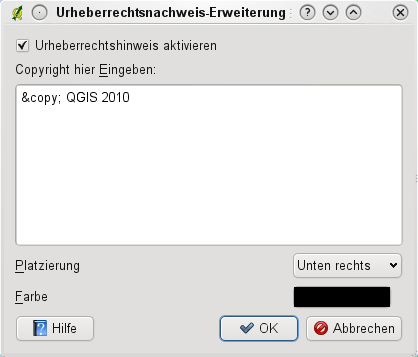
\includegraphics[width=0.6cm]{copyright_label}
 & Etiquette de copyright \index{extensions!copyright} & Afficher une étiquette de copyright avec les informations associées\\
\hline

\includegraphics[width=0.6cm]{diagram_overlay}
 & Diagramme de couche \index{plugins!diagram} & Placer des graphiques (camemberts, barres) ou des symboles proportionnels sur des couches vectorielles\\
\hline

\includegraphics[width=0.6cm]{dxf2shp_converter}
 & Convertisseur DXF2Shape \index{plugins!DXF2Shape} & Convertir un fichier au format DXF vers le format SHP\\
\hline
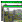
\includegraphics[width=0.6cm]{evis_icon}
 & eVis & Outil de Visualisation d'Événements\\
\hline

\includegraphics[width=0.6cm, height=0.6cm]{ftoolslogo}
 & fTools \index{plugins!ftools} & Une suite d'outils de recherche, d'analyse, de géométrie et de géotraitement\\
\hline
 & Outils GDAL \index{plugins!gdaltools} : interface graphique simplifiée pour les programmes de traitement raster GDAL\\
\hline

\includegraphics[width=0.6cm]{gps_importer}
 & Outils GPS \index{plugins!gps} & Charger et importer des données GPS\\
\hline

\includegraphics[width=0.6cm]{grass}
 & GRASS \index{plugin!grass toolbox} & Activer la puissante boîte à outils GRASS\\
\hline
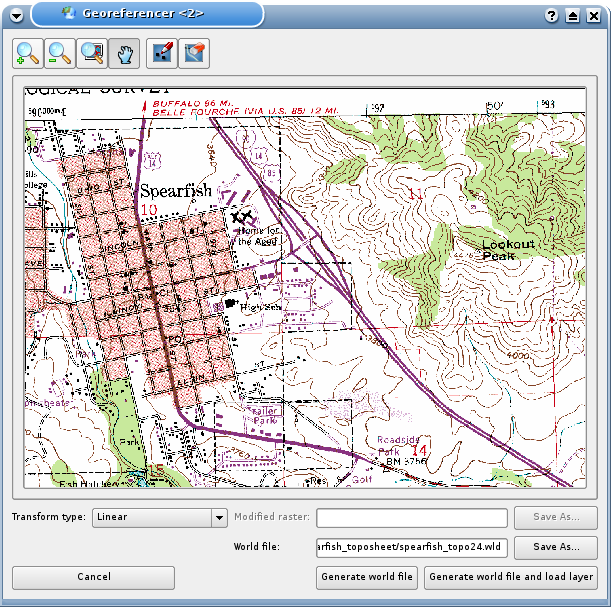
\includegraphics[width=0.6cm]{georeferencer}
 & Géoréférencer \index{plugin!georeferencer} & Ajouter des informations de projection aux fichiers raster\\
\hline

\includegraphics[width=0.6cm]{interpolation}
& Interpolation \index{plugins!Interpolation} & Interpolation sur la base de sommets d'une couche vectorielle\\
\hline

\includegraphics[width=0.6cm]{raster_terrain}
& Modelisateur de terrain \index{plugins!Raster Terrain Modelling} & Calculer la pente, l'aspect et la courbure totale des MNT\\
\hline

\includegraphics[width=0.6cm]{mapserver_export}
& Export MapServer \index{plugins!MapServer Export} & Exporter un projet \qg au format mapfile de MapServer\\
\hline
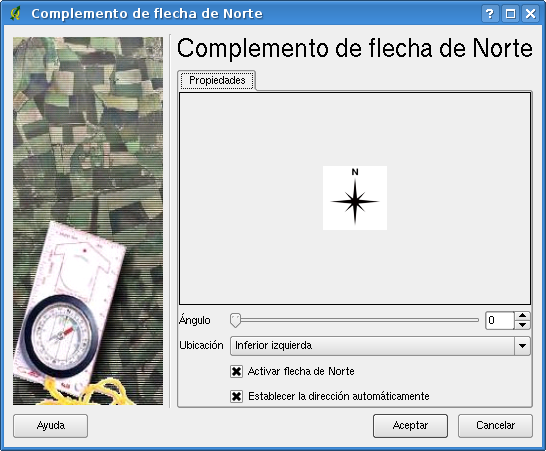
\includegraphics[width=0.6cm]{north_arrow}
& Flèche Nord \index{plugins!north arrow} & Afficher une rose des vents au premier plan de la carte\\
\hline

\includegraphics[width=0.6cm]{ogr_converter}
 & Convertisseur OGR \index{plugins!OGR converter} & Convertir les couches vectorielles dans les différents formats supportés par OGR\\
\hline
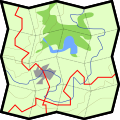
\includegraphics[width=0.6cm]{osm_icon}
 & OpenStreetMap & Visualiser et éditer des données OpenStreetMap\\
\hline

\includegraphics[width=0.6cm]{oracle_raster}
 & Georaster Oracle \index{plugins!georaster} & Accéder à des géorasters d'Oracle Spatial\\
\hline

\includegraphics[width=0.6cm]{plugin_installer}
 & Installateur d'extensions \index{plugins!Plugin Installer} & Télécharger et installer des extensions Python pour \qg\\
\hline

\includegraphics[width=0.6cm]{spiticon}
 & SPIT \index{plugins!spit} & Outil d'import de fichiers Shape vers PostgreSQL/PostGIS\\
\hline

\includegraphics[width=0.6cm]{quick_print}
 & Impression rapide \index{plugins!quick print} & Imprimer rapidement une carte avec un minimum d'efforts\\
\hline
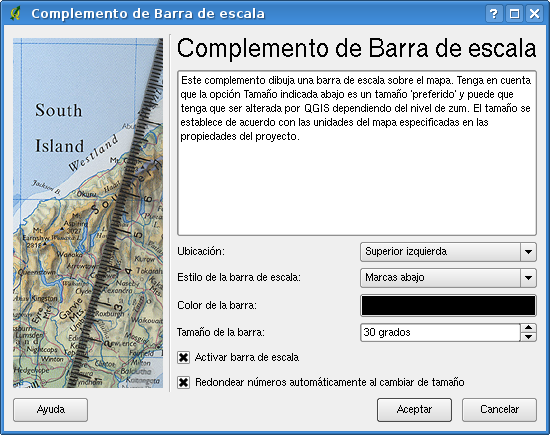
\includegraphics[width=0.6cm]{scale_bar}
 & Barre d'échelle \index{plugins!scalebar} & Afficher une barre d'échelle au premier plan de la carte\\
\hline

\includegraphics[width=0.6cm]{mIconAddWfsLayer}
 & WFS & Charger et afficher une couche WFS\\
\hline
\end{longtable}}

%\caption{Les extensions principales de \qg}\label{tab:core_plugins}
%\end{table}
